\documentclass{article}
\usepackage[left=2cm,right=3cm,top=2cm,bottom=3cm]{geometry}
\usepackage{amsmath}
\usepackage{verbatim}
\usepackage{hyperref}
\usepackage{tikz}

\begin{document}
\begin{center}
  \textbf{\LARGE Entropia de dados}\vspace{0.8cm}
  
  Kauan Toledo Camargo
\end{center}

\section{Database utilizada:}

Foi-se utilizado como base de dados qualitativos uma lista de jogos eletrônicos datados desde 1980 até 2023, contendo datas de lançamento, nota média e críticas. Neste trabalho iremos analizar a entropia das notas médias de usuários entre esses 1499 jogos.
\begin{center}
  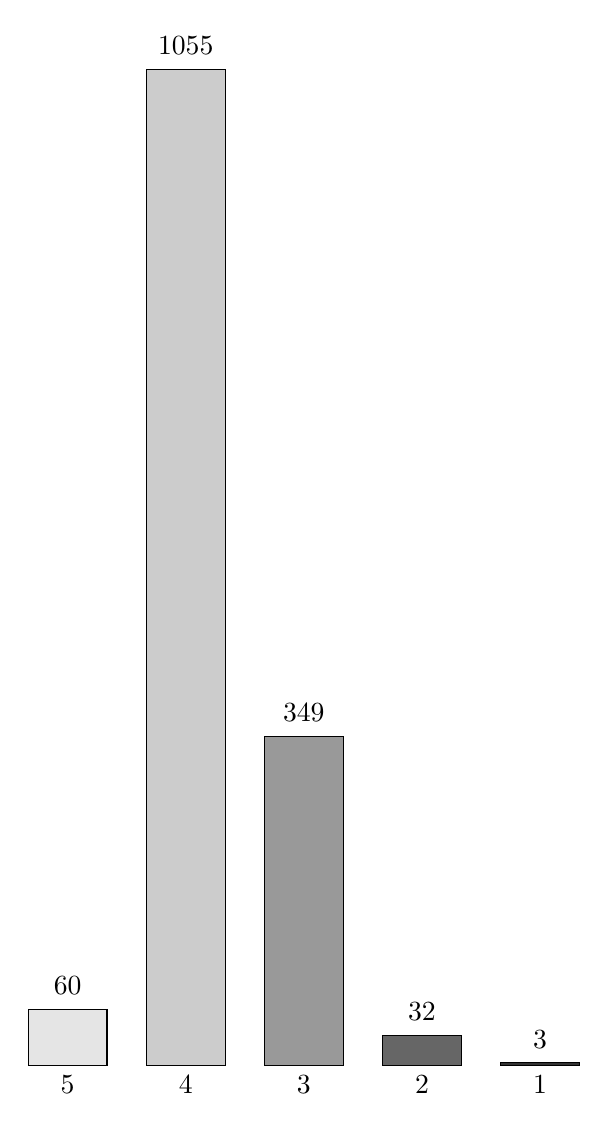
\begin{tikzpicture}
    % Define the data values
    \pgfmathsetmacro{\valueA}{60}
    \pgfmathsetmacro{\valueB}{1055}
    \pgfmathsetmacro{\valueC}{349}
    \pgfmathsetmacro{\valueD}{32}
    \pgfmathsetmacro{\valueE}{3}
  
    % Set the column width and spacing
    \pgfmathsetlengthmacro{\columnwidth}{1cm}
    \pgfmathsetlengthmacro{\columnspacing}{0.5cm}
  
    % Draw the columns
    \draw[fill=black!10!white] (0, 0) rectangle +(\columnwidth, 0.012 * \valueA);
    \draw[fill=black!20!white] (\columnwidth + \columnspacing, 0) rectangle +(\columnwidth, 0.012 * \valueB);
    \draw[fill=black!40!white] (2 * \columnwidth + 2 * \columnspacing, 0) rectangle +(\columnwidth, 0.012 * \valueC);
    \draw[fill=black!60!white] (3 * \columnwidth + 3 * \columnspacing, 0) rectangle +(\columnwidth, 0.012 * \valueD);
    \draw[fill=black!80!white] (4 * \columnwidth + 4 * \columnspacing, 0) rectangle +(\columnwidth, 0.012 * \valueE);
  
    % Add labels to the columns
    \node at (0.5 * \columnwidth, 0.012 * \valueA + 0.3) {\valueA};
    \node at (\columnwidth + 0.5 * \columnwidth + \columnspacing,0.012 * \valueB + 0.3) {\valueB};
    \node at (2 * \columnwidth + 0.5 * \columnwidth + 2 * \columnspacing, 0.012 * \valueC + 0.3) {\valueC};
    \node at (3 * \columnwidth + 0.5 * \columnwidth + 3 * \columnspacing, 0.012 * \valueD + 0.3) {\valueD};
    \node at (4 * \columnwidth + 0.5 * \columnwidth + 4 * \columnspacing, 0.012 * \valueE + 0.3) {\valueE};
  
    % Add axis labels
    \node[below] at (0.5 * \columnwidth, 0) {5};
    \node[below] at (\columnwidth + 0.5 * \columnwidth + \columnspacing, 0) {4};
    \node[below] at (2 * \columnwidth + 0.5 * \columnwidth + 2 * \columnspacing, 0) {3};
    \node[below] at (3 * \columnwidth + 0.5 * \columnwidth + 3 * \columnspacing, 0) {2};
    \node[below] at (4 * \columnwidth + 0.5 * \columnwidth + 4 * \columnspacing, 0) {1};
  \end{tikzpicture}
\end{center}

\begin{center}
  Os dados foram aredondados para facilitar o cálculo.\\
  \href{https://www.kaggle.com/datasets/arnabchaki/popular-video-games-1980-2023}{https://www.kaggle.com/datasets/arnabchaki/popular-video-games-1980-2023}
\end{center}

\pagebreak

\section{Calculando a entropia de dados}

\begin{align*}
  P&(nota5)=\frac{60}{1499}=0.04\\
  P&(nota4)=\frac{1055}{1499}=0.704\\
  P&(nota3)=\frac{349}{1499}=0.233\\
  P&(nota2)=\frac{32}{1499}=0.021\\
  P&(nota1)=\frac{3}{1499}=0.002\\
\end{align*}

\begin{align*}
  H(X) =& -\sum_{i=1}^{n} P(x_i) \log_2 P(x_i)\\
  H(X) =&-(0.04 \log_2 0.04 + 0.704 \log_2 0.704 + 0.233 \log_2 0.233\\
        &+ 0.021 \log_2 0.021 + 0.002 \log_2 0.002)\\
  H(X) =&-(0.04 (-4.644) + 0.704 (-0.506) + 0.233 (-2.102)\\
        &+ 0.021 (-5.573) + 0.002 (-8.966))\\
  H(X) =&1.168
\end{align*}

\begin{align*}
  H_{max} =& log_2 5\\
  H_{max} =& 2.322
\end{align*}

\textbf{Conclusão:} Os dados possuem um grau médio de aleatoridade, se distanciando de forma moderada da distribuição uniforme comparados com a entropia máxima possível.

\pagebreak

\section{Python - entropy.py}

\textbf{\large Código:}

\begin{verbatim}
  import math

  entropy = 0.0
  total = 0
  classes = []
  n = int(input('Quantidade de classes: '))

  for i in range(n):
    classes.append(int(input(f"Valor da classe {i+1}: ")))
    total += classes[i]

  for i in range(n):
    probability = classes[i] / total
    entropy -= probability * math.log2(probability)

  maxEntropy = math.log2(n)

  print(f'Valor Total: {total}')
  print(f'Entropia dos dados: {entropy:.3f}')
  print(f'Entropia máxima: {maxEntropy:.3f}')
\end{verbatim}

\textbf{\large Console:}

\begin{verbatim}
  Quantidade de classes: 5
  Valor da classe 1: 3 
  Valor da classe 2: 32
  Valor da classe 3: 349
  Valor da classe 4: 1055
  Valor da classe 5: 60
  Valor Total: 1499
  Entropia dos dados: 1.168
  Entropia máxima: 2.322
\end{verbatim}

\vspace{\fill}

\begin{center}
  \href{https://github.com/Lazy-Machine/DataEntropy}{https://github.com/Lazy-Machine/DataEntropy}
\end{center}

\end{document}